\newpage
\section{Beschreibung der Module}
	\subsection{Kurbeschreibung}
	Das gesamte Projekt besteht auf folgenden Modulen (Flussdiagramme sind im Kapitel~\ref{Module}):
	\begin{description}[font=\sffamily\bfseries, leftmargin=1.5cm,style=sameline] 
	\item{\textbf{main}}
	Dies ist das Hauptprogramm. Beim Start werden die serielle Schnittstelle und das \textbf{scheduler}-Modul initialisiert. Das Konsolenprozess wird erzeugt. Timer-Interrupts werden initialisiert. Danach befindet sich das Hauptprogramm in einer Endlosschleife.
	
	\item{\textbf{proc\_console}}
	Dies ist der Konsolenprozess. Der Prozess ist eine Endlosschleife, welche die Eingaben von der seriellen Schnittstelle abholt. Diese Eingaben werden auf �bereinstimmung mit den bekannten Befehlen gepr�ft. Unbekannte Eingaben werden verworfen. Befehle werden erkannt und ausgef�hrt.
	\item{\textbf{scheduler}} Dies ist der eigentliche Task-Verwalter. Das Modul besteht aus Subroutinen:
	\begin{description}[font=\sffamily\bfseries, leftmargin=0.5cm,style=sameline] 
	\item{\textbf{new\_proc}}
		Hier wird ein neuer Prozess erzeugt. In der Prozesstabelle im externen RAM wird nach dem ersten freien Platz gesucht (first fit). Jeder Prozess wird vereinfacht gleich gro� angenommen.
		Die Position des gefundenen freien Platzes in der Prozesstabelle entspricht einer Position vom Datenbereich der Prozesse. Die Datenbereiche werden initialisiert.
		
	\item{\textbf{del\_proc}} Hier wird der Verweis auf den Datenbereich eines zu beendenden Prozesses aus der Prozesstabelle entfernt. Hiermit kennt der Task-Verwalter diesen Prozess und seinen Datenbereich nicht mehr.
	
	\item{\textbf{change\_proc}}
	Hier wird der Kontext der Prozesse getauscht. Hierbei werden alle prozessrelevanten Daten in den externen Speicher ausgelagert (�hnlich wie Swapping). N�chster Prozess wird aus der Prozesstabelle geholt und sein Kontext wird ins RAM geladen.
	
	\end{description} 
	
	\item{\textbf{serial}} Dieses Modul stellt Routinen zum I/O auf der seriellen Schnittstelle bereit.
	
	\item{\textbf{proc\_a}} Prozess a: Eine Zeichenfolge \textquotedblleft abcde\textquotedblright wird auf der seriellen Schnittstelle 0 ausgegeben.
	\item{\textbf{proc\_b}} Prozess b: Gibt jede Sekunde \textquotedblleft+\textquotedblright auf die serielle Schnittstelle aus
	\item{\textbf{proc\_z}} Prozess z: Ruft fkt\_text auf
	\item{\textbf{fkt\_text}} Testprozess: gibt eine Zeichenfolge auf serielle Schnittstelle 1 aus.
	\end{description}
	
\newpage
\subsection{Speichernutzung und Variablen}

F�r das Programm werden folgende Speicherbereiche reserviert und verwendet:

\subsubsection*{Variablen und Konstanten}

Variablen und Konstanten werden im \textquotedblleft variables.inc\textquotedblright{} dem Befehl \begin{center}
<NAME> EQU <HEX>
\end{center} angelegt. Durch einbinden der Datei in jedes Modul sind die Variablen global bekannt. Die genaue Beschreibung der Variablen und deren Funktion ist einem  kommentierten Listing im Anhang zu entnehmen.

\subsubsection{Externer Datenbereich}
Externer Datenbereich wird folgenderma�en genutzt. Zu Beginn des Programms werden zwei Datenbereiche im externen Speicher reserviert. Ein Bereich ist die Prozesstabelle. Pro Prozess sind hier 4 Byte vergeben. Die setzen sich wie folgt zusammen. 2 Byte DPTR auf den dazugeh�rigen Prozessdatenbereich, 1 Byte Bitmaske mit Prozessstatus und Prozesstyp und 1 Byte f�r die Prozess ID.

Es sind insgesamt 20 Prozesse m�glich. Die Entscheidung f�r die Zahl 20 ist willk�rlich und kann auch generell auf \textquotedblleft beliebig\textquotedblright{} gesetzt werden. Die Grenze bildet hier die Gr��e des externen Datenbereichs. 

Jeder Prozess besitzt seinen eigenen Datenbereich, worin sein Kontext aufbewahrt wird. Pro Prozess sind 32 Byte reserviert. Aktuell werden lediglich 23 Byte benutzt. 10 Byte f�r den Stack und 13 Byte f�r den geforderten Kontext. Eine Erweiterung der Stackgr��e ist m�glich. Abbildung~\ref{fig:ext_data} zeigt die Speicherbelegung. 
\begin{figure}[H]
\centering
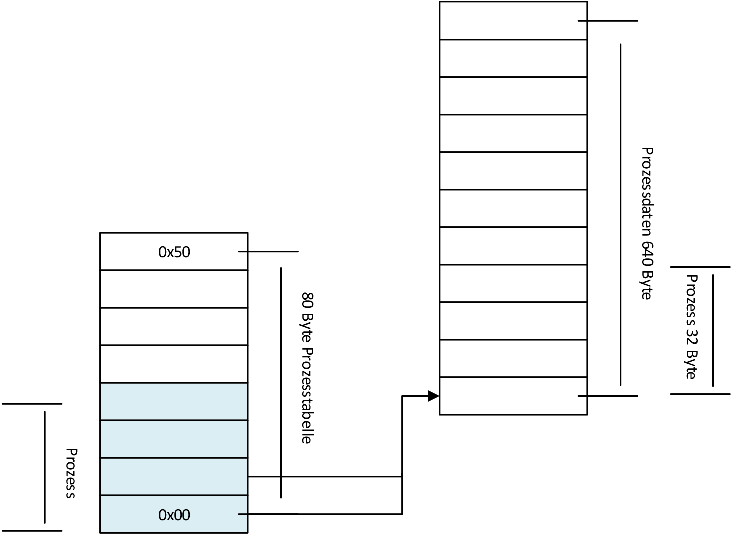
\includegraphics[width=0.7\textwidth]{./images/ext_data}
\caption{Speicherbelegung des externen RAM}
\label{fig:ext_data}
\end{figure}

\subsection{Module\label{Module}}
\subsubsection{Hauptmodul \texttt{main.a51}}
In der Abbildung~\ref{fig:main} ist das Ablaufdiagramm vom Hauptmodul dargestellt. Die genaue Beschreibung der einzelnen Operationen ist aus dem Listing im Anhang zu entnehmen.

\begin{figure}[H]
\centering
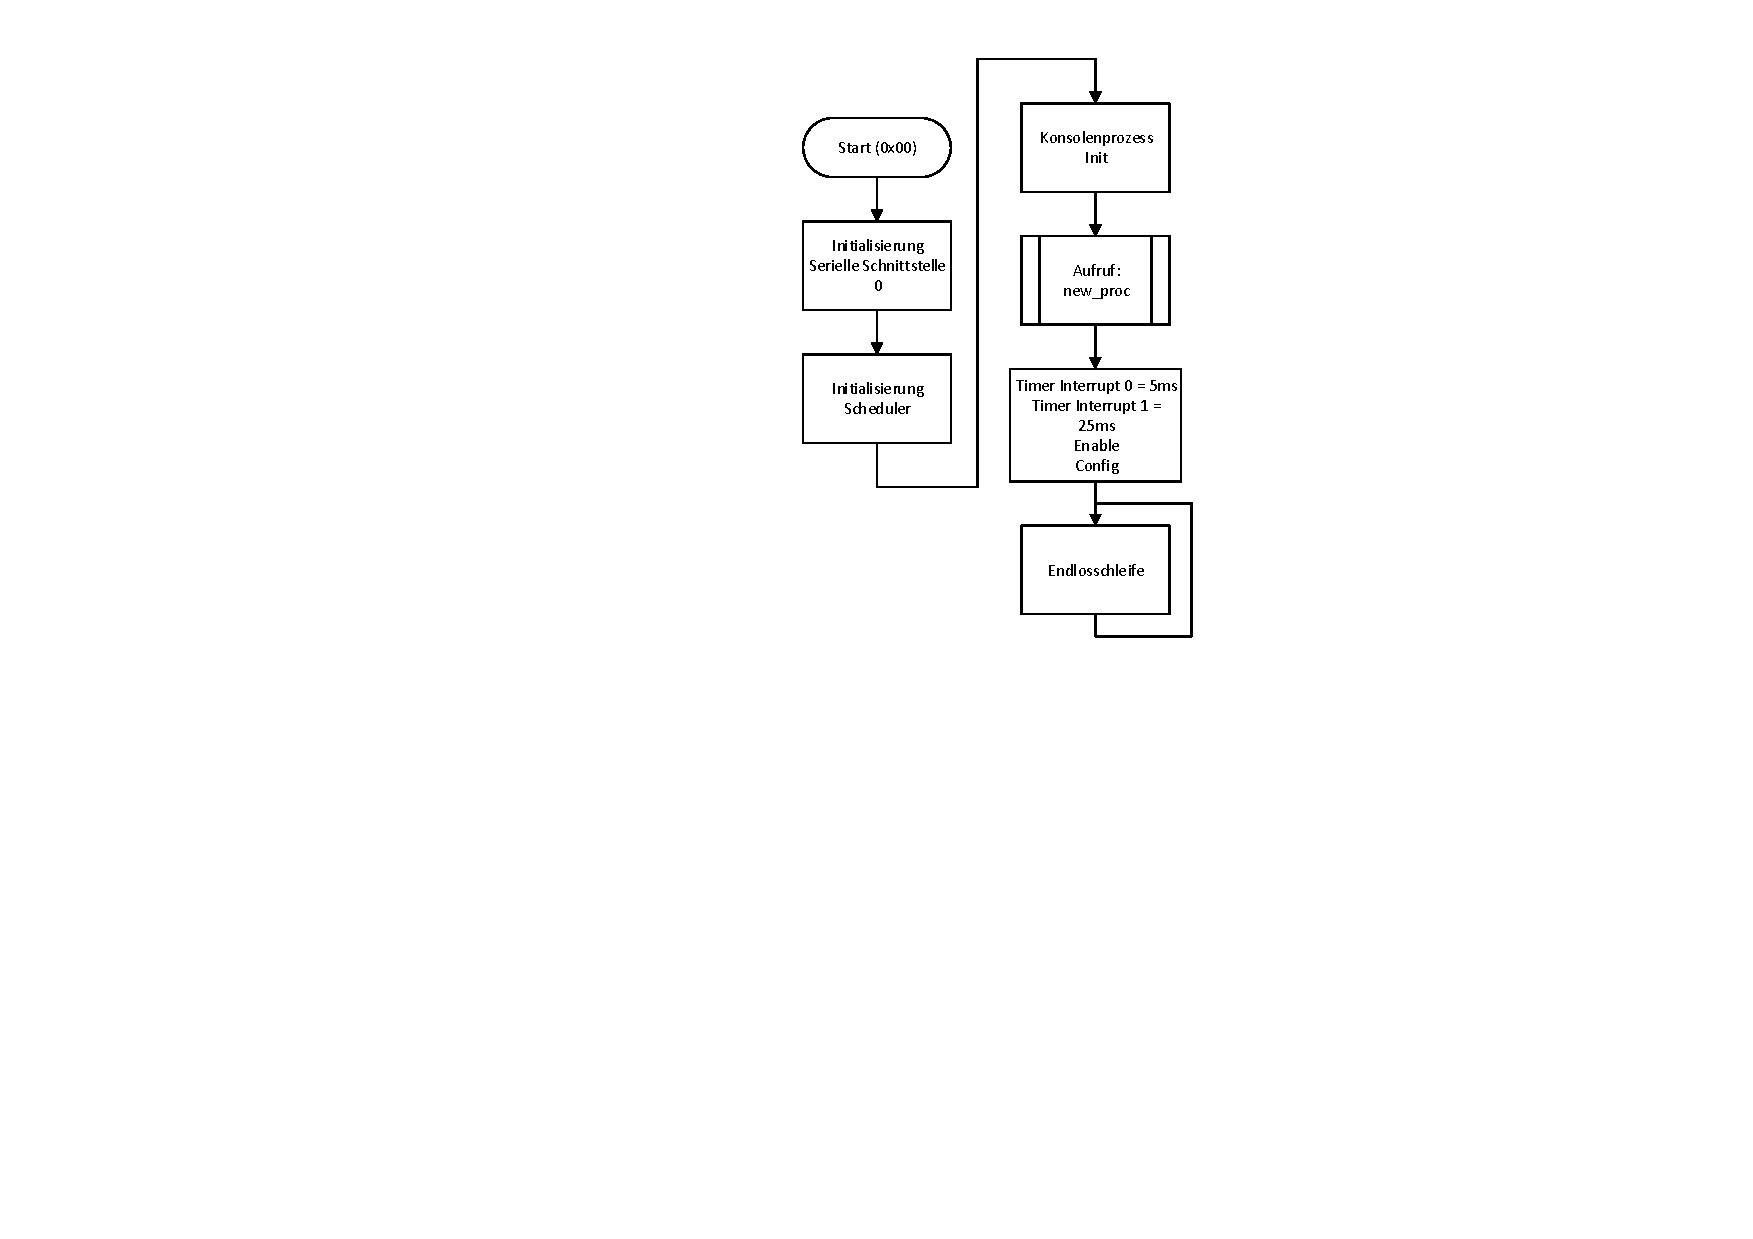
\includegraphics[width=0.5\textwidth]{./images/main}
\caption{Ablaufdiagramm main.a51}
\label{fig:main}
\end{figure}

\subsubsection{Konsolenprozess \texttt{proc\_console.a51}}
In der Abbildung~\ref{fig:console} ist das Ablaufdiagramm vom Hauptmodul dargestellt. Die genaue Beschreibung der einzelnen Operationen ist aus dem Listing im Anhang zu entnehmen.
\begin{figure}[H]
\centering
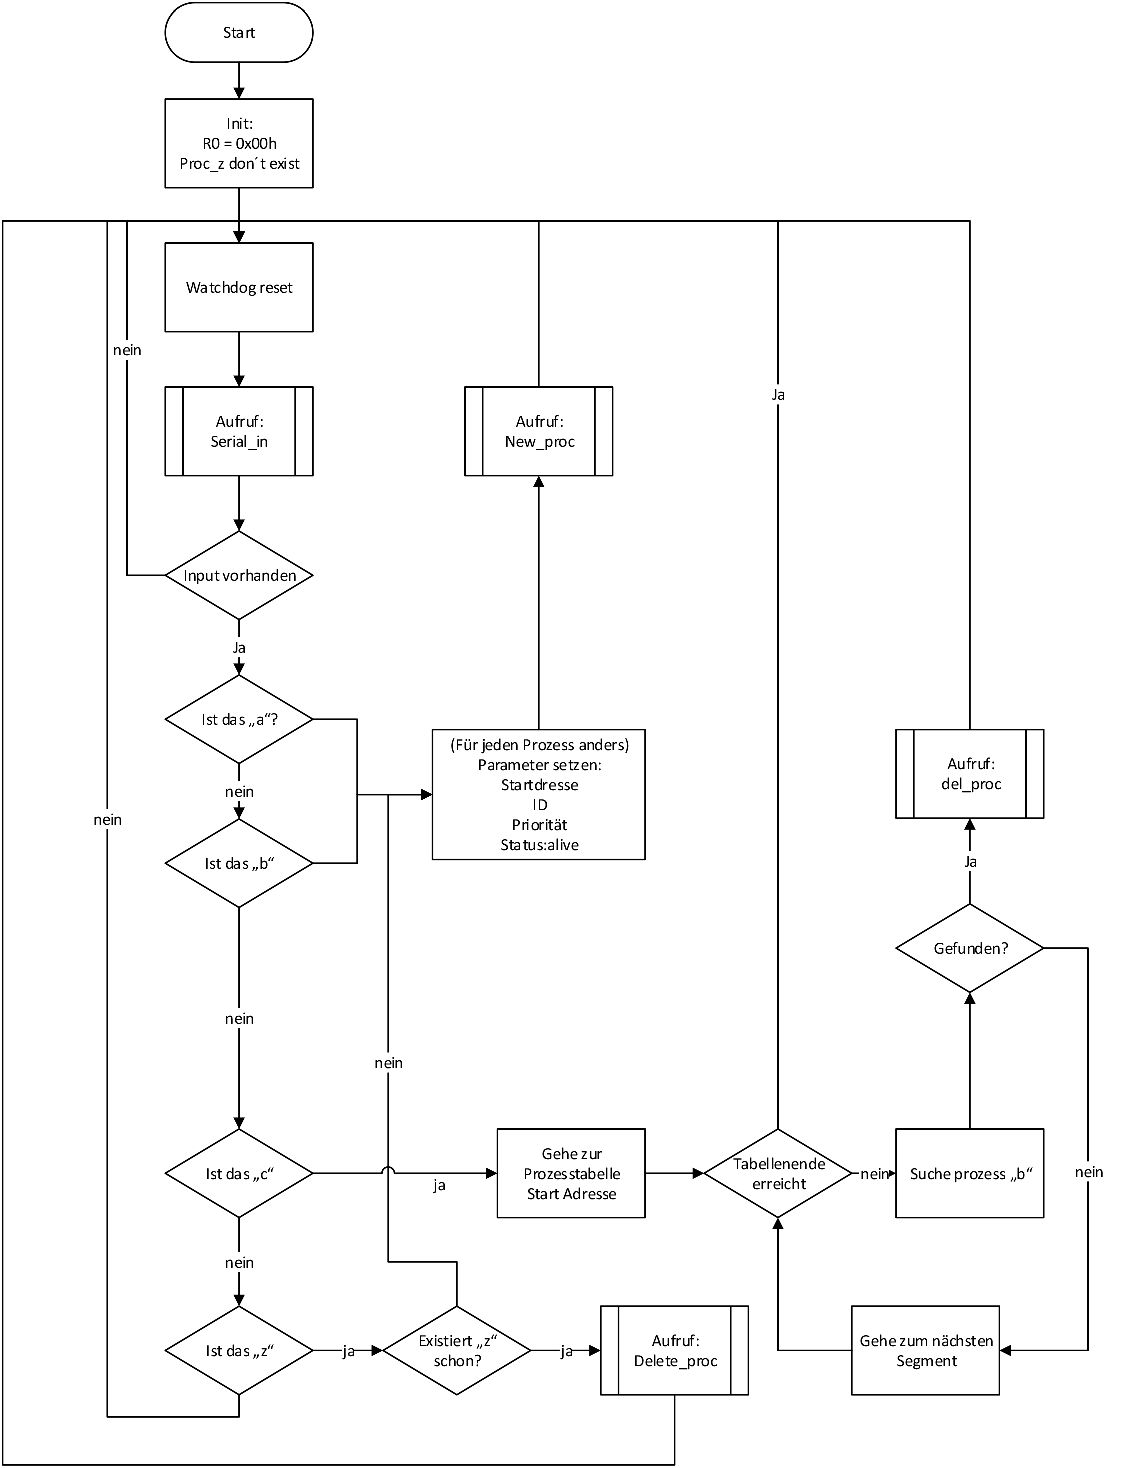
\includegraphics[width=\textwidth]{./images/console}
\caption{Ablaufdiagramm \texttt{proc\_console.a51}}
\label{fig:console}
\end{figure}
\newpage
